% Template for ICIP-2022 paper; to be used with:
%          spconf.sty  - ICASSP/ICIP LaTeX style file, and
%          IEEEbib.bst - IEEE bibliography style file.
% --------------------------------------------------------------------------
\documentclass{article}
\usepackage{spconf,amsmath,graphicx}

\usepackage[section]{placeins}
\usepackage{float}

% Example definitions.
% --------------------
\def\x{{\mathbf x}}
\def\L{{\cal L}}

% Title.
% ------
\title{Learned image compression}
%
% Single address.
% ---------------
\name{Juha Ylikoski, Teemu Eerola, Nardos Estifanos}
\address{juha.ylikoski@tuni.fi, teemu.eerola@tuni.fi, nardos.estifanos@tuni.fi}
%
% For example:
% ------------
%\address{School\\
%	Department\\
%	Address}
%
% Two addresses (uncomment and modify for two-address case).
% ----------------------------------------------------------
%\twoauthors
%  {A. Author-one, B. Author-two\sthanks{Thanks to XYZ agency for funding.}}
%	{School A-B\\
%	Department A-B\\
%	Address A-B}
%  {C. Author-three, D. Author-four\sthanks{The fourth author performed the work
%	while at ...}}
%	{School C-D\\
%	Department C-D\\
%	Address C-D}
%
\begin{document}
%\ninept
%
\maketitle
%
\begin{abstract}
Image compression has had some major new ideas in forms of learned image compression. 
Especially the neural network based learned image compression methods have achieved even better performance than the more traditional manually designed lossy image compression models.
These new methods are not without their own problems. The large neural network based models can achieve remarkable compression ratios and perceived image quality, but have suffered widely form being too computationally expensive to be usable.

In this work we are reviewing and trying to replicate one of these methods which claims good quality, compression ratio and speed.
\end{abstract}
%
\begin{keywords}
Learned image compression, ELIC Efficient Learned Image Compression
\end{keywords}
%

\setcounter{section}{-1}

\section{Authors' contributions}

\section{Introduction} % Juha
\label{sec:intro}
With the rise of cloud services and mobile devices, the amount of stored digital media has grown rapidly. 
Large part of this data is stored images which take considerable amount of space.
Traditionally these images have been compressed or encoded to formats like jpeg or png which compress the images and usually lose some details (lossy compression).
With the rise of neural networks and machine learning there has been many attempts to achieve higher compression ratios and lose less details.
Many of these methods have achieved higher compression ratio with better perceived image quality and less visible artifacts but have been prohibitively expensive in terms of computational cost.

This work tries to replicate paper ELIC: Efficient learned image compression with unevenly grouped space-channel contextual adaptive coding \cite{ELIC} which has introduced an efficient learned image compression method (ELIC) which fairs well in the benchmarks and is also reasonable in terms of computational cost.
The model is based on multiple convolutional neural networks which encode the image into latent space.
This latent representation is then passed into autoencoder which compresses it and is sent to the receiver. 
The autoencoder takes as parameters input from a model they call Space-Channel ConTeXt (SCCTX).
This model optimizes the encoding/decoding parameters of Gaussian encoder to minimize the redundancy in both channel dimension and in spatial dimension to further reduce the number of bits transferred.

The output of the arithmetic decoder is passed into otherwise identical neural network as the first one in the pipeline, but in reversed order of layers with transposed convolutional layers instead of convolutional layers.
The output of this network is now our final image output. 

There are still some limitations to this approach. 
One of which is that the network input image size is limited.
This means that the network cannot take as input arbitrarily sized images but of course these images can be padded or split or cropped and inputted to the network in multiple pieces.
Second limitation of this network is the amount of time it takes to encode an image and decode an image. 
Even when it is considerably faster than other learned image compression methods, in our testing it still very slow and instead of highlighted 100 microseconds for a image which size was not specified, when we tried to encode and compress an 1024x2048 sized image it took approximately 4 seconds for encoding and 5 seconds for decoding.
Most likely our implementation has many problems which would cause this value to be far away from the highlighted one, but we are about 4 magnitudes away from their highlighted value which at least to us raises some questions.


\section{Related Works}
\label{sec:related_works}
Recently, in learned compression, we have seen the proliferation of deep learning-based image compression techniques using automatic coding architectures with great success and promising results. The development of previous learning-based compression models has spanned several years, hence, there are many related works. 

In the early stages, some work was proposed to perform non-differential quantization and rate estimation for complete training, for instance, some works focused on developing network structures that can obtain more compact and efficient latent images and reconstruct high-quality images from compressed images. 

It is noted that traditional image compression techniques, such as JPEG and BPG, have limitations in terms of subjective quality and rate-distortion performance. Learned image compression techniques have shown promise in addressing these limitations by approaching it as rate-distortion optimization problem \cite{ELIC}.

\begin{equation}
    R + \lambda \cdot D
\end{equation}

Some approaches include content weighting strategies or combining of different channels using principal component analysis, or consider energy compression or use deep residual devices to improve the network architecture \cite{balle2016}. Recently, several studies have investigated adaptive contextual entropy estimation models to guide the optimization process of neural network parameters to achieve an optimal trade-off between reconstruction error and required bits (entropy), including \cite{AgustssonEirikur2017SVQf, balle2018, mbt2018, LeeJooyoung2019CEMf} Entropy estimation methods have greatly improved learning compression algorithms, and the most representative methods are hyperprior models and joint models.


Several recent works that have made significant contributions to the field of learned image compression. One such work is the \cite{VincentPascal2008Eacr, TheisLucas2017Licw, balle2016} End-to-End Optimized Image Compression (EOIC) model, which uses a convolution neural network (CNN) to compress images. EOIC uses a combination of entropy coding and arithmetic coding to achieve high compression rates. Another work is the Generative Adversarial Networks (GAN)-based image compression model, which uses a GAN to generate compressed images. GAN-based models have shown promise in improving the subjective quality of compressed images.

The use of attention mechanisms in learned image compression models is also another discussion. Attention mechanisms allow the model to focus on specific regions of the image that are important for compression. One such model is the Attention Recurrent Network for Image Compression (ARNIC) \cite{XueYuyang2019ABIC}, which uses a recurrent neural network (RNN) with an attention mechanism to compress images. Attention mechanisms have shown promise in improving the rate-distortion performance of learned image compression models.

Another important improvement comes from the use of residual blocks in learned image compression models \cite{balle2016}. Residual blocks are a type of neural network layer that allows for the reuse of features learned in previous layers. They have shown promise in improving the rate-distortion performance of learned image compression models. They are also easier to extend for dynamic or slimmable inference, while other techniques like GDN require special handling.

Learning from these techniques have shown promise in improving the rate-distortion performance of learned image compression models. It is proposed to make use of uneven channel-conditional adaptive coding, motivated by the observation of energy compaction in learned image compression.

\section{Methodology}
\label{sec:methods}
\subsection{architecture}
\label{sec:architecture}
In this work, we adopted the ELIC-sm model architecture, which is a significantly smaller model that full ELIC architecture presented in Figure \ref{fig:architecture}. The differences to ELIC are in main transform networks $g_a$ and $g_s$ where ELIC-sm do not implement attention blocks and have only 1 residual block sequentially connected rather than 3 in full ELIC. The architecture of the implemented model is described in table \ref{table:architecture} following table 2 of ELIC paper supplementary material \cite{ELIC}. In the table 5x5 denotes the kernel size 5, s2 the stride in convolution to be 2 and the last symbol in each row presents the number of output channels. 

\begin{figure*}[h!]
    \centering
    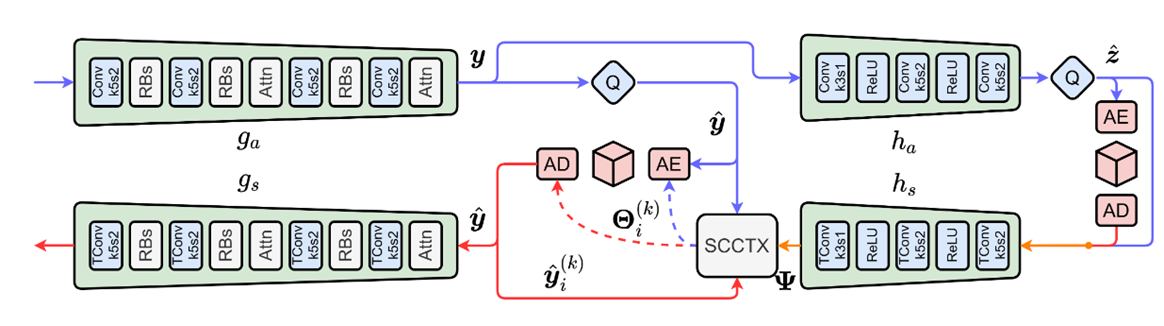
\includegraphics[width=7in]{architecture.png}
    \caption{Architecture of full ELIC \cite{ELIC}. The
blue and red arrows denote the encoding and decoding data flow. The orange ones are shared by both encoding and decoding.}
    \label{fig:architecture}
\end{figure*}

\begin{table}[!h]
\label{table:architecture}
\begin{center}
\caption{Architecture of ELIC-sm main transform networks. \cite{ELIC}}
\begin{tabular}{l|l}
\hline
Analyzer $g_a$ & Synthesizer $g_s$ \\
\hline
in: 3-channel image & in: M-channel symbols \\
\hline
Conv 5 $\times$ 5, s2, N & TConv 5 $\times$ 5, s2, N \\
ResBottleneck$\times$1 & ResBottleneck$\times$1 \\
Conv 5 $\times$ 5, s2, N & TConv 5 $\times$ 5, s2, N \\
ResBottleneck$\times$1 & ResBottleneck$\times$1 \\
Conv 5 $\times$ 5, s2, N & TConv 5 $\times$ 5, s2, N \\
ResBottleneck$\times$1 & ResBottleneck$\times$1 \\
Conv 5 $\times$ 5, s2, M & TConv 5 $\times$ 5, s2, 3 \\
\hline
\end{tabular}
\end{center}
\end{table}

We chose the smaller ELIC-sm architecture to reduce the amount of computational complexity and the need for data. We also kept the hyperparameters $M$ and $N$ reasonably low to further ease the training of the model. $M$ controls the number of channels in latent space and $N$ the number of channels in main transform networks. We leverage the ready-made implementation of Gaussian and arithmetic en/de-coders from CompressAI library \cite{compressai}. 

\subsection{Space-Channel Context model}
In works previously that ELIC \cite{ELIC} the context models were used only to predict either parameters of channel wise or spatial context to encode/decode pixels \cite{balle2016, mbt2018, balle2018, checkerboard}. The proposed method in ELIC uses both channel and spatial information in context model to predict the parameters $\mathbf{\Theta_i^{(k)}}$of next group \cite{ELIC}. 

The channel groups are formed in uneven manner based on observation that most of the energy is often concentrated on early channels. Therefore, the number of channels in groups is rising towards latter groups. The context prediction is made using all previous channel groups combined. When encoding or decoding the first channel group the channel wise context is therefore set to zeros. Because the uneven groups the sizes of inputs and outputs of the channel context model changes over the groups, and therefore separate model is implemented for each group. The number of networks is one less than number of groups because the networks make prediction of the next group parameters. The architecture of channel-wise context model is implemented as it is from the ELIC paper. \cite{ELIC} We doubled the number of channels only in the last convolutional layer.

The spatial context can be implemented as autoregressive convolution where each pixel prior to the current pixel must be predicted \cite{mbt2018}. A more efficient approach to implement spatial context prediction as checkerboard convolution introduced by He \textit{et al.} 2021 \cite{checkerboard}. The concept involves dividing the group into half like picking only the white or black squares from checkerboard and making predictions to these anchor pixels first. Another half of the group, the non-anchors, can be then predicted using the firstly encoded/decoded group as context. In the prediction of anchor parameters, the spatial context is simply set to zeros. The architecture of spatial context module is implemented with one checkerboard convolution layer with kernel size of 5 and stride of 1 that keeps the number of channels the same. 

The combined representation of prediction parameters is got from parameter aggregation network that combines the spatial and channel wise context predictions with hyperprior $\mathbf{\Psi}$ from hyperparameter synthetization network $h_s$. Because of uneven sizes of channel groups, channel and spatial context prediction networks, a separate networks needs to be implemented for each group. Architecture of parameter aggregation network is implemented as it is in the ELIC paper figure 6 with linear reduction of channels in layers \cite{ELIC}. 

The table \ref{table:SCCTX} shows the number of trainable parameters in thousands of SCCTX for channel number of $M=192$ and the default channel block sizes $(16,16,32,64,M-128)$ from the ELIC paper. The channel context model parameters for block$_0$ is \textit{NaN}, because it does not exists due to reasons discussed earlier. 

\begin{table}[!h]
\label{table:SCCTX}
\begin{center}
\caption{Number of trainable parameters in SCCTX in\\ thousands for each block ($b_i$) and for each component.}
\begin{tabular}{c c c c c c c} 
 \hline
  & $b_0$ & $b_1$ & $b_2$ & $b_3$ & $b_4$ & sum \\
 \hline\hline
 channel & \textit{NaN} & 26 & 103 & 410 & 512 & 1050 \\
 \hline
 spatial & 13 & 13 & 51 & 205 & 205 & 487 \\
 \hline
 par.agg. & 198 & 198 & 277 & 480 & 480 & 1632 \\
 \hline
 sum & 210 & 236 & 431 & 1095 & 1197 & 3169 \\
 \hline
\end{tabular}
\end{center}
\end{table}

\subsection{Training versus compression flow}
The inference and training procedures differ from each other due to the undifferentiable nature of encoders. In inference time we want to compress the image to actual discrete bitstream and in training we want to just get the likelihoods from the entropy models and retain the gradient information. The gradient can be retained from the encoders by not compressing the image to bitstream, but just adding gaussian noise to image to mimic the effect of quantization. The approach was presented by \cite{balle2016}. 
With the checkerboard spatial context model another shortcut can be made in training time to further reduce the computational complexity of training. Following the work of He \textit{et al.} 2021 \cite{checkerboard} we used one pass encoding in training where parameters of non-anchor blocks are calculated from the input without calculating the parameters of anchor blocks. This approach was different from that presented in ELIC paper \cite{ELIC}, where they encoded $y+mu$ to bitstream instead of $y$ and therefore one pass encoding was not possible. We did not follow the implementation of ELIC because of lack of understanding about entropy models.

At inference time we calculate a separate bitstream to each image in batch sequentially and leverage the full context prediction by first decoding the anchor blocks and then the non-anchor blocks. This still allows us to decode the channel blocks in the image separately using the features of entropy model. However, for practical use cases, the batch processing should be allowed to benefit from the parallel computation capabilities of GPUs.

\section{Experiments}
\label{sec:experiments}
\subsection{Training} % Juha
\label{sec:training}

Training of the model was done with 6000 largest images from ImageNet \cite{imagenet} which were randomly cropped into size of 16x16 pixels.
These images were then run through the forward method of the network.
The forward method of the network does not fully compress the images but it transforms them into the latent spaces and the loss function takes into account the likelihood of good compression ratio as well as mse loss.

The model was trained with multiple different configurations. We tried $\lambda \in \{0.0008, 0.001\}$ where latent space channels $M$ and $N$ were $M=N=192$ and $\lambda \in \{0.0004, 0.0008\}$ where latent space channels $M$ and $N$ were $M=192, N=128$.
All of these models were trained for approximately 300 epochs but they could be still trained further.
Unfortunately due to lack of computational capabilities we could not train more networks and even these networks most likely could have been trained for longer but with epochs taking from 180 seconds (for smaller latent space) to 300 seconds (larger latent space), we could not train them further due to time constraints.

After obtaining different models with different parameters, we have calculated the PSNR and MS-SSIM \cite{Bjntegaard2001CalculationOA, WangZhou2003Mssf} values to plot the rate-distortion curve which helps in visualizing the performance of compression as well as perceived quality and bits used to represent an image compared to each other and other techniques such as JPEG. For this evaluation, we have modified the script from compressai \cite{compressai} to get close enough comparison with other techniques, and made use of KODAK\cite{kodak} and CLIC professional \cite{clic} datasets.


\section{Results}
\label{sec:results}

In Figure a, we demonstrate the reconstruction performance of the four models trained with different parameters.

\begin{table}[!h]
\label{table:models}
\begin{center}
\begin{tabular}{c c c}
    Row (Model) 1: epoch=250 & $\lambda$=8e-4 & N=M=192 \\
    Row (Model) 2: epoch=300 & $\lambda$=4e-4 & N=128, M=192 \\
    Row (Model) 3: epoch=300 & $\lambda$=8e-4 & N=128, M=192 \\
    \textbf{Row (Model) 4}: epoch=300 & $\lambda$=1e-2 & N=M=192 \\
\end{tabular}
\end{center}
\end{table}

\pagebreak

\begin{figure}[h!]
\begin{minipage}[b]{0.8\linewidth}
    \centering
    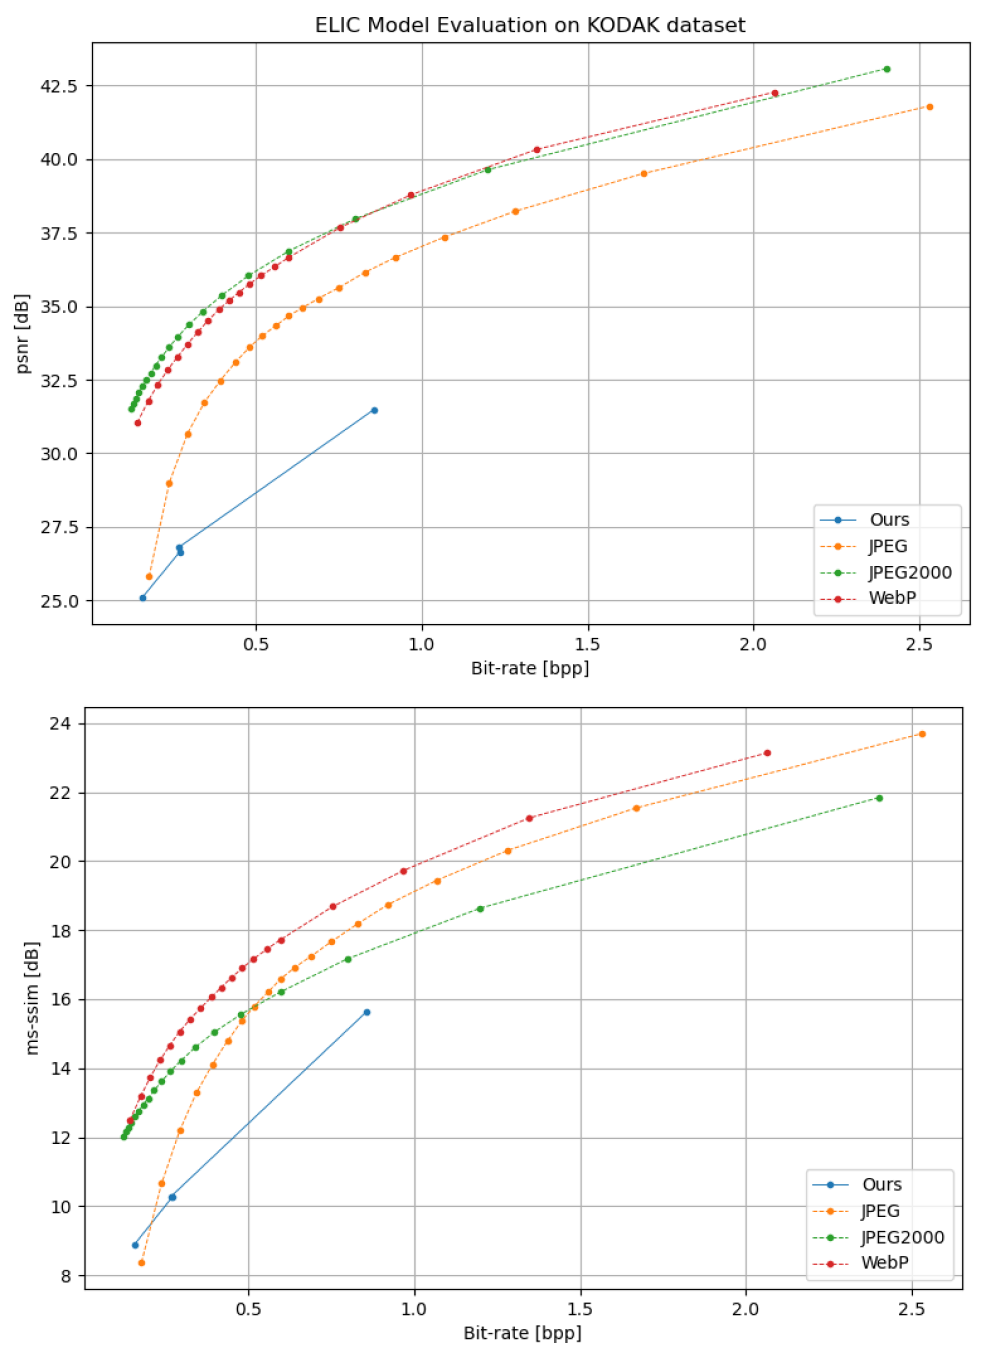
\includegraphics[width=7.2cm]{kodak_fixed.png}
    \centerline{(a) Average values.}\medskip
\end{minipage}
\begin{minipage}[b]{0.8\linewidth}
    
    \centering
    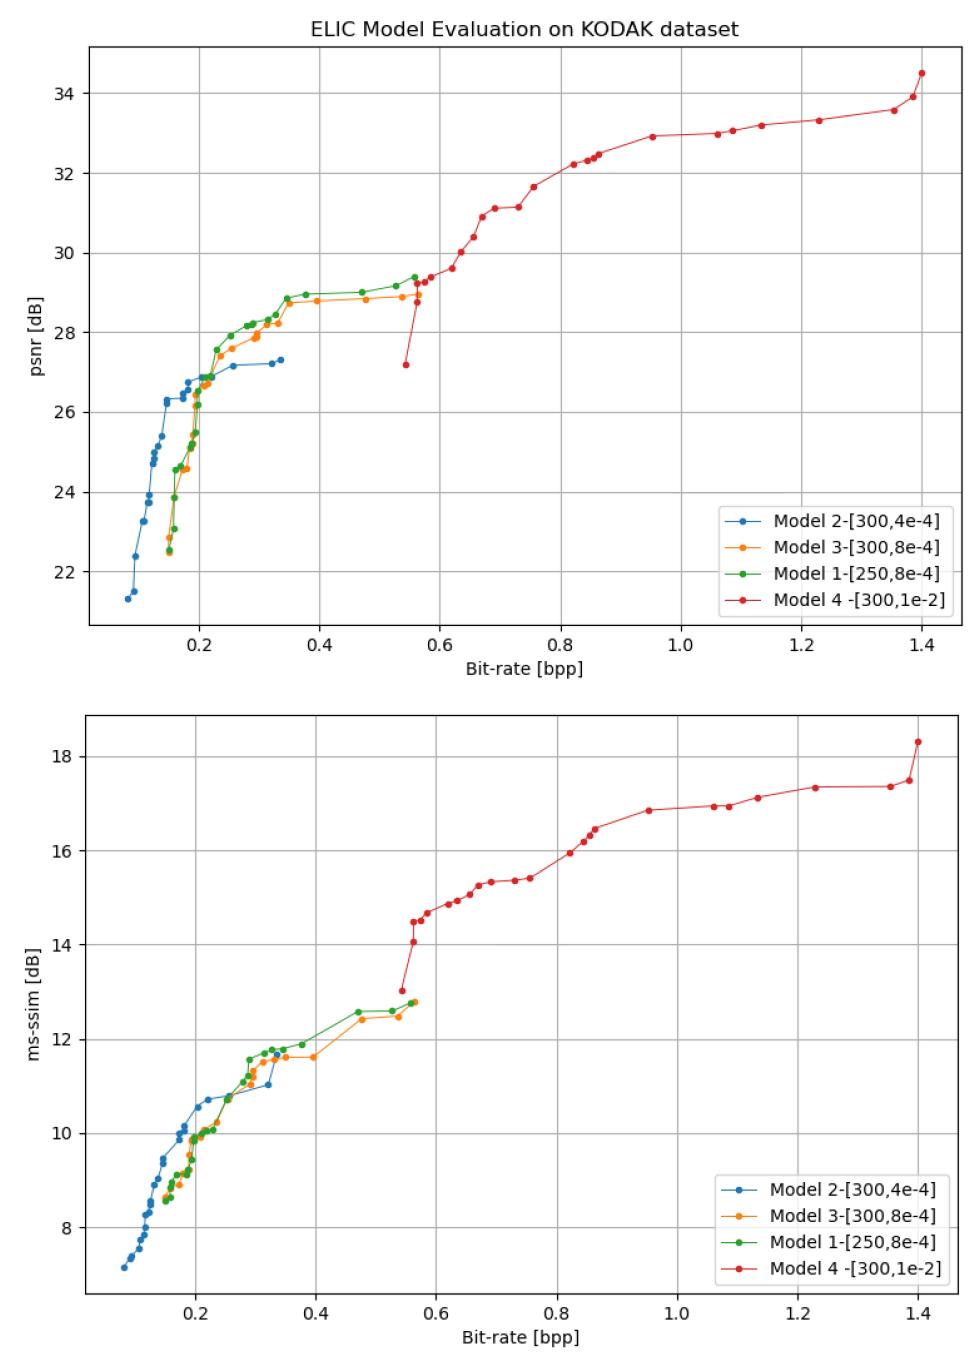
\includegraphics[width=7.2cm]{kodak_per_fixed.png}
    \centerline{(b) Performance on individual images.}\medskip
\end{minipage}
    \label{fig:results}
    \caption{Results on KODAK dataset \cite{kodak}.}
\end{figure}

\pagebreak

\begin{figure*}[h!]
\centering
\begin{minipage}[b]{.8\linewidth}
    \centering
    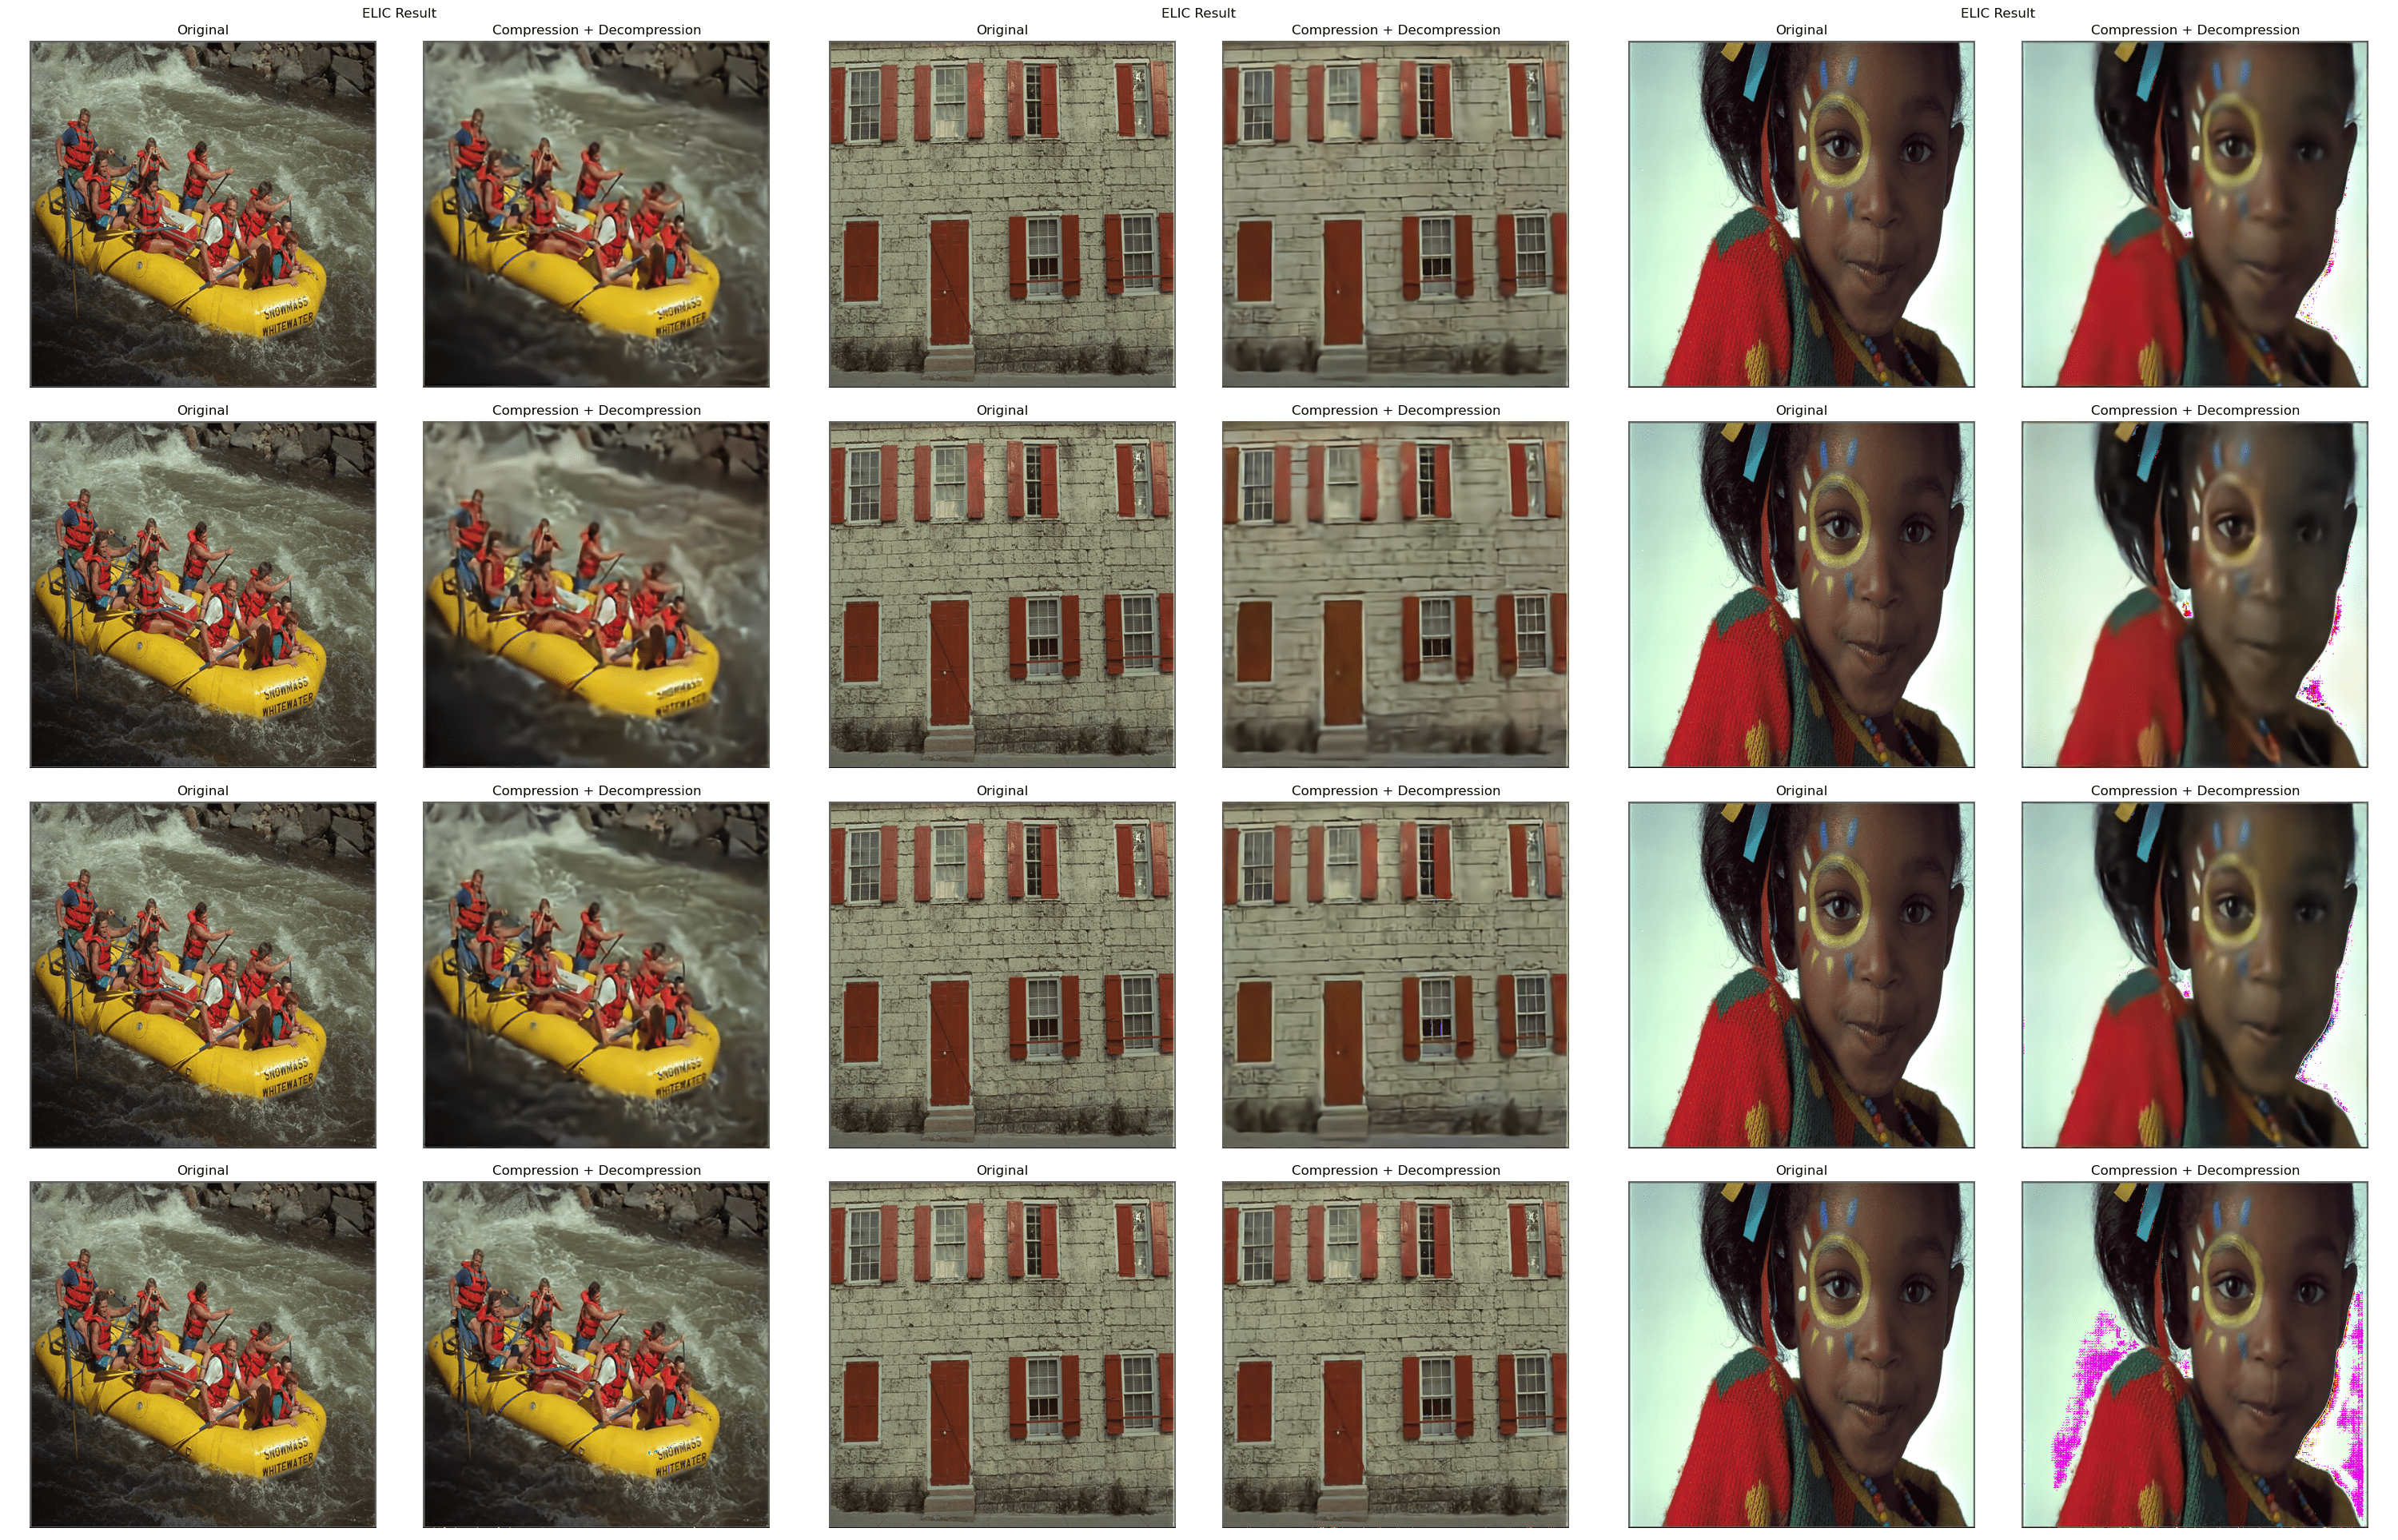
\includegraphics[width=\linewidth]{reconstruction.png}
    \centerline{(a)  Result images from our models. Each row is results from the model 1 to 4 respectively}\medskip

\end{minipage}
\begin{minipage}[b]{.5\linewidth}
    \centering
    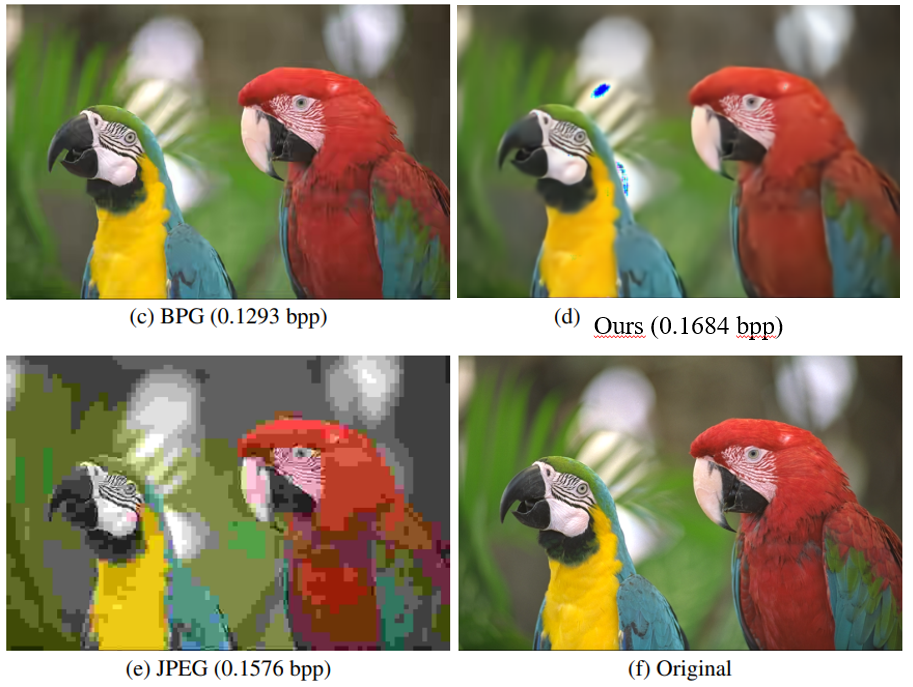
\includegraphics[width=\linewidth]{comparison.png}
    \centerline{(b) Comparisons to conventional image compression methods JPEG and BPG to our results from Model 3 and original image.}\medskip
\end{minipage}
    \caption{Result/comparison images.}
    \label{fig:images}
\end{figure*}

\vfill\pagebreak
\vfill\pagebreak


\section{Discussions and Conclusions}
The goal of this work was to implement and verify the methods of He \textit{et al.} 2022 \cite{ELIC} for learned image compression. We successfully implemented and trained 4 different models targeted to low compression ratios by varying the model hyperparameters $M$, $N$ and $\lambda$ in loss function. The implementation differs from the paper in few details as discussed earlier. Due to limited time and computing resources we were not able to train our models to convergence and we used fewer images in our training set. Finetuning of the models using MS-SSIM as loss function was also discarded due to computation and time restrictions. 

The results from our models were far from the level of original ELIC paper in terms of subjective and objective measurements in quality. This was caused by implementation differences and different training setups. Additionally, our models suffer from color artifacts that were introduced in various areas in result images. We are not sure what is the cause of these artifacts, but possible reasons are errors in implementation for example overflow in data types or underfitted models. In subjective evaluation we were able to pass the level of JPEG compression, but objective metrics were orders of magnitude behind JPEG. We can conclude that were where able to have working image compression models using methods introduced by He \textit{et al.} 2022 \cite{ELIC} in ELIC, but we can not confirm the improved quality and inference speed they achieved. We neither studied the progressive decoding or the fast thumbnail generator introduced in original paper. 

Apparently the models from original ELIC paper also suffers from some kind of artifacts that they do not mention in paper. In successive work He \textit{et al.} 2022 \cite{PO-ELIC} propose a discriminator network in top of ELIC to reduce amount of know artifacts in learned image compression with Generative adversarial network (GAN) inspired training. Other interesting directions in learned image compression are purely GAN and diffusion based compressors, that are capable of reconstructing even unseen areas of image using techniques of generative methods \cite{HIFIC, diffusion}. 



% References should be produced using the bibtex program from suitable
% BiBTeX files (here: strings, refs, manuals). The IEEEbib.bst bibliography
% style file from IEEE produces unsorted bibliography list.
% -------------------------------------------------------------------------
\bibliographystyle{IEEEbib}
\bibliography{strings,refs}

\end{document}
